\documentclass{article}
\setlength{\parindent}{0cm}
\usepackage{mathtools}
\usepackage{amssymb}
\usepackage{amsthm}
\title{Analysis of the Efficacy of Squarified and Knife Tree Maps}
\author{Ben Lewin, Ilan Gray, Philip Braunstein (a.k.a Braun and Blew)}
\date{November 24, 2014}
\begin{document}
\maketitle
\abstract{
Squarified Tree Maps (SQTM) and Knife Tree Maps (TM) are two visualizations used to represent hierarchical data.
We hypothesized that it is easier for people to accurately estimate relative areas in TMs
as opposed to SQTMs, we also hypothesized that accuracy on TM estimation would be correlated with SQTM estimation. We developed visualizations and tested them on 12 subjects. We found that TMs induce less error as expected. These results were statistically significant to a 90\% confidence threshold with a p--value of 0.084 on the Welch Two-Sample Test. Both TM and
SQTM error distributions followed the normal distribution with p--values from the Shapiro-Wilk Test of 0.119 and 
0.165, respectively. Finally, we found that an individual's TM accuracy and SQTM accuracy are not correlated with an $R^2$
value of 0.0731. Further studies include increasing the sample size of the experiment and testing truly 
hierarchical data. 
}

\section*{Introduction}
Hierarchical data is frequently generated in this world; however, this is an ornery form of data to visualize. Two solutions
suggested to display hierarchical data are Knife Tree Maps (TM) and Squarified Tree Maps (SQTM). Both types of tree maps divide a rectangular area into rectangles whose areas are correlated with some piece of data. TM visualizations
start divide the first level of the given area into vertical slices and the next level into horizontal slices. Vertical and horizontal
slices continue to alternate for each level of hierarchy. SQTM visualizations attempt to make the most square-like segments
of areas using the aspect ratio.\\

We wanted to explore how each of these visualizations handles hierarchical data at \emph{each level}. Thus, we used
nonhierarchical data to simulate estimating areas within a single level of hierarchy. We made this choice to attempt to establish the preeminence  of TMs over SQTMs in nonhierarchical data before working with truly hierarchical data. Indeed, we hypothesized that TMs present relative areas more clearly than SQTMs\\

The most straight forward hypothesis is that if a person is good at accurately interpreting one visualization, that person will
also be good at accurately interpreting a different type of visualization. In order to shed light on the validity of this hypothesis,
we ran a linear regression on each subject's average scores for the TM and SQTM error scores. We expected these data to be
strongly correlated.

\section*{Methods}
\subsection*{Subject Testing}
Subjects were recruited from two pools - P.Braunstein's roommates and people in Halligan. The visualization testing
framework from Lab 5 was adapted to test TM and SQTM visualizations. The two rectangles to compare were indicating
by hi-lighting these rectangles blue (the rest of the rectangles had a white background). Each subject was tested with 15 total visualizations. The type of each visualization was determined by Processing's inborn random number generator.  

\subsection*{Data Analysis}
Data analysis was performed using R and Microsoft Excel. The Clevland McGill Error was used to determine accuracy for each visualization. Error bars indicate 95\% confidence. The Shapiro-Wilk Test was used to determine whether the errors calculated for each chart type (TM and SQTM)
followed a normal distribution. The Welch Two-Sample Test was used to determine if the TM and SQTM error distributions
were statistically significant distributions. Since only two visualizations were used, a Bar Graph was used to plot the error. This was a stylistic decision. Each subject's average Clevland McGill Error for each type of visualization. The average TM error and the average SQTM were plotted (x values were TM score and y values were SQTM score for each subject). A linear regression was performed in Excel to determine the correlation. All other statistical tests were performed using the native R functions.

\section*{Results}
\subsection*{TMs Moderately Better than SQTMs}
TM Clevland McGill Eror was $2.18 \pm 0.332$, and SQTM Clevland McGill Error was $2.56 \pm 0.259$. These values including
the error bars are shown in \textbf{Figure 1}.

\begin{figure}
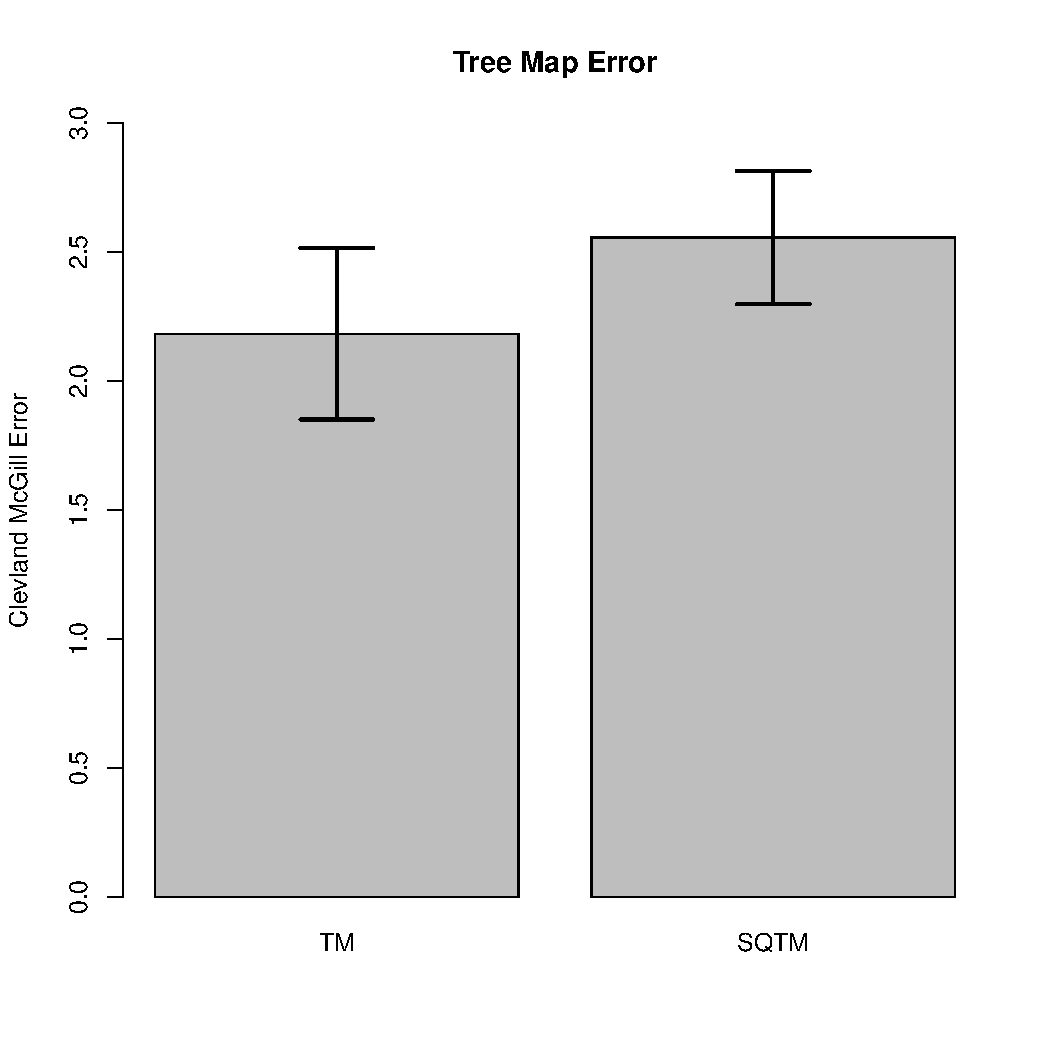
\includegraphics[width=0.9\textwidth]{mapsBarPlot.pdf}
\caption{Clevland McGill Error}
\end{figure}

\subsection*{TMs and SQTMs Follow the Normal Distribution}
Both the TM and SQTM errors were found to follow a normal distribution using the Shapiro-Wilk Test. The TM p-value was 0.119, and the SQTM p-value was 0.165. Both of these p-values were even above the very liberal p-value cutoff of 0.1. Since, these
p-values failed to prove the null hypotheses incorrect, these distributions are normal. The TM W Statistic was 0.977, and the SQTM W Statistic was 0.979.

\subsection*{Statistically Different Distributions to 90\%}
The Welch Two-Sample Test between the TM errors and the SQTM errors generated a t statistic of -1.74 with 168 degrees of freedom. These were used to determine a p-value of 0.0844. This p-value proves that the TM and SQTM error distributions are
different to 90\% confidence. However, these data were not statistically significant to prove these two distributions distinct to the
industry standard 95\% confidence. 

\subsection*{TM and SQTM Analysis Prowess Not Correlated}
A subject's ability to effectively understand TMs was found not to be correlated to the subject's ability to effectively understand SQTMs. The $R^2$ value of the linear regression was 0.0731 (see \textbf{Figure 2}).

\begin{figure}
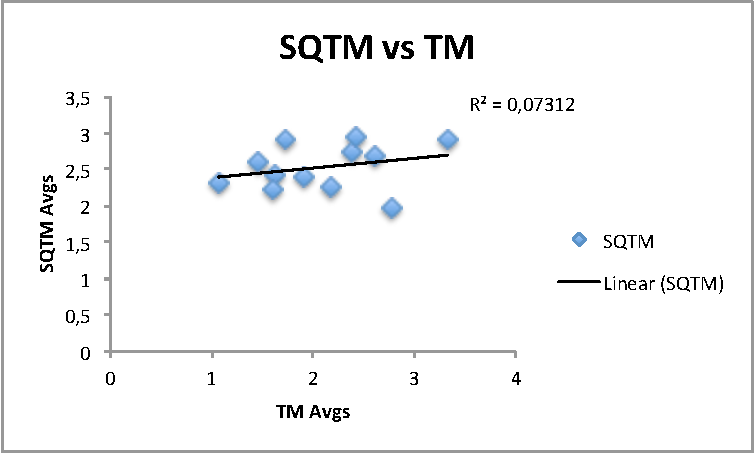
\includegraphics[width=0.9\textwidth]{sqtmvstm.pdf}
\caption{TM and SQTM Linear Regression}
\end{figure}

\section*{Conclusions and Future Directions}
This study shows that TMs are significantly better than SQTMs to 90\% confidence. This confirms our first hypothesis. However, we believe that testing a larger sample size (50-100 subjects) would demonstrate this to 95\% confidence or greater. An expanded study with greater sample size would be necessary to establish the true statistical significance of this finding. \\

We were surprised to find that successfully estimating areas on a TM was \emph{not} correlated with successfully estimating areas on an SQTM. Thus, our second hypothesis was proven incorrect. \\

We believe that this study demonstrates that on \emph{each level} of hierarchy, the TM is a better visualization than the SQTM. In other words, the TM is a better visualization than SQTM for nonhierarchical data. A future study would involve a similar setup with truly hierarchical data.
\end{document}